\chapter{Supersymmetry}
\begin{section}{Natural Supersymmetry}

Supersymmetry (SUSY) is an extension of the Standard Model that introduces a new symmetry that relates fermionic and bosonic degrees of freedoms~\cite{ref:hierarchy1,ref:hierarchy2,Ramond:1971gb,Golfand:1971iw,Neveu:1971rx,Volkov:1972jx,Wess:1973kz,Wess:1974tw,Fayet:1974pd,Nilles:1983ge}.
This symmetry imposes that for every fermionic degree of freedom in the Standard Model, there exists a ``superpartner'' bosonic degree of freedom, and vice versa.
Furthermore, this symmetry dictates that both sets of particles couple to physics at the $\Lambda_{UV}$ scale identitically.

In the Minimal Supersymmetric Standard Model (MSSM)~\cite{Csaki:1996ks}, the Standard Model is extended to include a Higgs sector comprised of two scalar doublets and only the SM superpartners.
The superpartners of fermions are scalars and labeled by prefixing an ``s'' to the beginning of the corresponding SM particle name, while the superpartners of bosons are spin-1/2, labeled by suffixing an ``ino'' to the end of the corresponding SM particle name, and collecticely known as gauginos.
Thus, the SUSY particles consist of 4 higgsinos, 12 squarks, 9 sleptons, and 7 gauginos, where there are 2 scalar particles for each SM fermion in order to preserve the number of degrees of freedom.
The superpartners of SM particles are not necesarily mass eigenstates and can mix.
The gauge and mass eigenstates of the superpartners, along with their properties, are shown in Table~\ref{tab:susy_particles}.

\begin{table}[tb!]
\centering
\renewcommand{\arraystretch}{1.25}
\begin{tabular}{|c|c|c|c|c|}
\hline
Name                       &  Spin                &  Gauge Eigenstates                                            &  Mass Eigenstates \\
\hline
\hline  
Higgs bosons               &  0                   &  $H^0_u$ $H^0_d$ $H^+_d$ $H^-_d$                              &  $h^0$ $H^0$ $A^0$ $H^\pm$ \\
\hline
\multirow{3}{*}{squarks}   &  \multirow{3}{*}{0}  &  $\tilde{u}_L$ $\tilde{u}_R$ $\tilde{d}_L$ $\tilde{d}_R$      &  same \\
                           &                      &  $\tilde{c}_L$ $\tilde{c}_R$ $\tilde{s}_L$ $\tilde{s}_R$      &  same \\
                           &                      &  $\tilde{t}_L$ $\tilde{t}_R$ $\tilde{b}_L$ $\tilde{b}_R$      &  $\tilde{t}_1$ $\tilde{t}_2$ $\tilde{b}_1$ $\tilde{b}_2$\\
\hline
\multirow{3}{*}{sleptons}  &  \multirow{3}{*}{0}  &  $\tilde{e}_L$ $\tilde{e}_R$ $\tilde{\nu}_e$                  &  same \\
                           &                      &  $\tilde{\mu}_L$ $\tilde{\mu}_R$ $\tilde{\nu}_\mu$            &  same \\
                           &                      &  $\tilde{\tau}_L$ $\tilde{\tau}_R$ $\tilde{\nu}_\tau$         &  $\tilde{\tau}_1$ $\tilde{\tau}_2$ $\tilde{\nu}_\tau$\\
\hline
neutralinos                &  1/2                 &  $\tilde{B}^0$ $\tilde{W}^0$ $\tilde{H}^0_u$ $\tilde{H}^0_d$  &  $\tilde{N}_1$ $\tilde{N}_2$ $\tilde{N}_3$ $\tilde{N}_4$\\
\hline
charginos                  &  1/2                 & $\tilde{\Wboson}^\pm$ $\tilde{H}^+_u$ $\tilde{H}^-_d$         &  $\tilde{C}^\pm_1$ $\tilde{C}^\pm_2$ \\
\hline
gluino                     &  1/2                 & $\glu$                                                        &  same \\
\hline
\end{tabular}
\renewcommand{\arraystretch}{1}
\caption{The additional SUSY particles in the Minimal Supersymmetric Standard Model.}
\label{tab:susy_particles}
\end{table}

With the addition of these superpartners, a mechanism for naturally cancelling the radiative corrections to the Higgs mass is apparent, as the Higgs will couple to these new massive particles as well and provide additional radiative corrections that cancel the SM contributions.
For example, for a fermion $f$, the radiative corrections from the corresponding sfermion $\tilde{f}$, shown in Figure~\ref{fig:higgs_scalar_loop}, take the form
\begin{align}
\delta \mh^2|_{\tilde{f}} = &+N_{\tilde{f}}\frac{\lambda_{\tilde{f}}}{8\pi^2} \left[-\Lambda^2_{UV} + 2m_{\tilde{f}}^2\ln\left(\frac{\Lambda_{UV}}{m_{\tilde{f}}}\right)\right] \nonumber \\
                            &-N_{\tilde{f}}\frac{\lambda_{\tilde{f}}}{8\pi^2} \left[-2m_f^2 + 4m_f^2\ln\left(\frac{\Lambda_{UV}}{m_{\tilde{f}}}\right)\right] + \mathcal{O}(\frac{1}{\Lambda^2_{UV}})
\end{align}
using the relation $\sqrt{2}m_f = \lambda_f\nu$.
Supersymmetry imposes that $N_{\tilde{f}} = N_f$ and $\lambda_{\tilde{f}} = -\lambda_f^2$, and thus, in the case where $m_f = m_{\tilde{f}}$, this perfectly cancels not only the quadratic divergence in Equation~\ref{eqn:higgs_fermion_correction} but also the higher-order corrections, solving the Hierarchy and Naturalness Problems.

\begin{figure}[tbp!]
\begin{center}
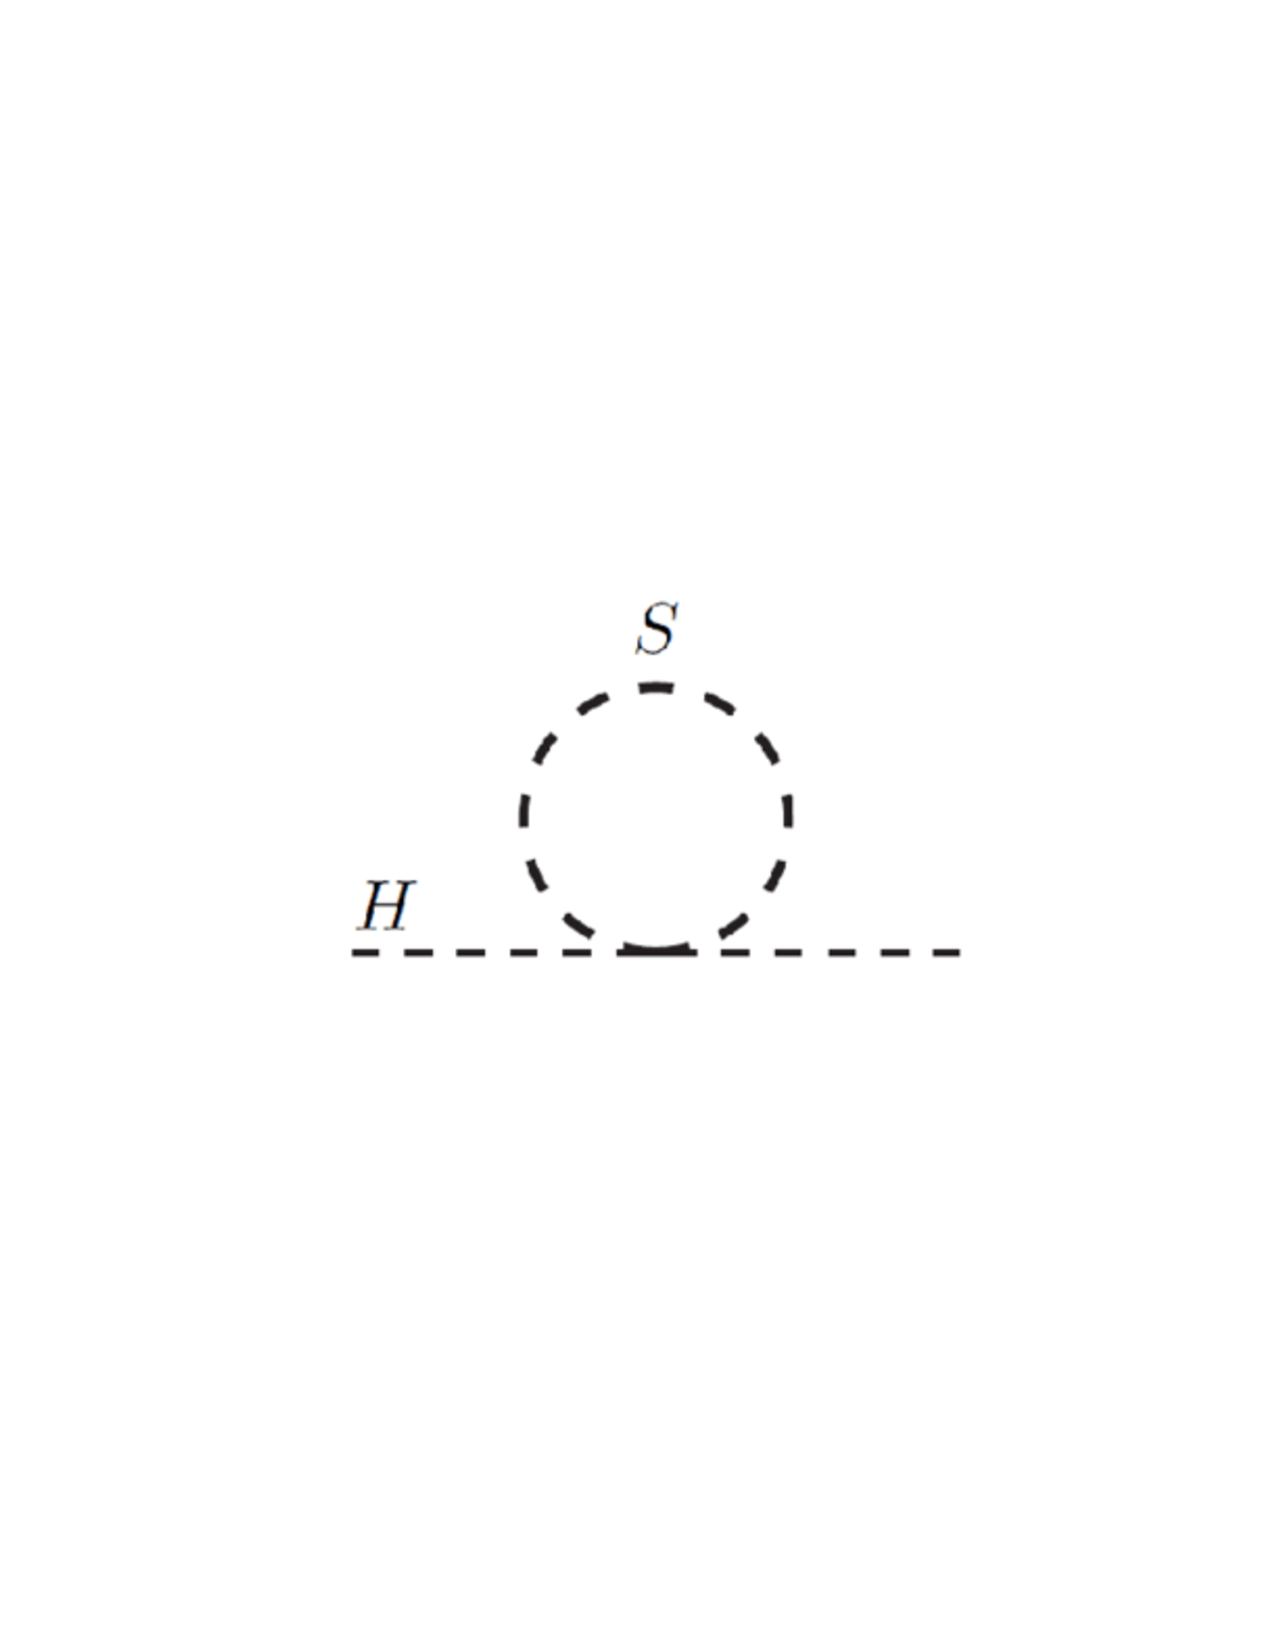
\includegraphics[angle=0,width=0.60\columnwidth]{fig/higgs_scalar_loop.pdf}
\end{center}
\caption{The scalar one-loop Higgs mass correction.}
\label{fig:higgs_scalar_loop}
\end{figure}

Of course, no superparticles have been observed at the SM scale.
This, however, does not imply that supersymmetry is incorrect but only that it may be a broken symmetry.
In this scenario where $m_f \neq m_{\tilde{f}}$, the quadratically divergent terms still cancel and what is left is only a lograithmic divergence, mediated by the squared mass difference of the partner particles:
\begin{align}
\delta \mh^2 = N_f\frac{\lambda_f^2}{8\pi^2} \left(m_f^2 - m_{\tilde{f}}^2\right) \ln\left(\frac{\Lambda_{UV}}{m_{\tilde{f}}}\right) + ...\ .
\label{eqn:total_higgs_correction}
\end{align}
This squared mass difference defines the degree to which the Higgs mass is fine-tuned.

\end{section}

\begin{section}{Phenemonological and Experimental Constraints}
\label{sec:susy_constraints}

While there is no theoretical prediction for the mass of the supersymmetric particles, there are certain guidelines for what the scale of these masses should be for a given level of fine-tuning that is deemed acceptable.
Firstly, the Higgsino masses are directly controlled by the value of $\mu$, which is related to the electroweak scale by
\begin{align}
-\frac{m_{\Zboson}}{2} = \mh^2 + |\mu|^2,
\end{align}
indicating that the Higgsino masses must be near the electroweak scale, $\sim 100~\GeV$, in order avoid a large fine-tuning of parameters.

The other superparticle masses are constrained by the size of their contributions to the Higgs mass, described in Equation~\ref{eqn:total_higgs_correction}.
Not all superparticles, however, contribute equally to the Higgs mass, and thus the phenemonological constraints for paritcles are in proportion to the size of their correction to the Higgs mass.
The largest constraint is on the stop squark masses due to the large Yukawa coupling of the top quark, which implies that the stop masses must be relatively light in order to keep the squared mass difference small and correspondingly the overall contribution small.
This also constrains the mass of the left-handed sbotom squark as it is in a doublet with $\tilde{t}_L$ and thus must not be much heavier.
Finally, the gluino couples to the squarks at the one-loop level, which means it still couples to the Higgs boson at the two-loop order, despite the Yukawa coupling for a gluon being zero.
This constraint on the gluino is looser than for other particles described, but since it is strongly interacting, it has a high cross section at the Large Hadron Collider (LHC) and is thus an important experimentally accessible particle.
Not considering model-dependent concerns, these are generically the only SUSY particles that are required to be light, and the rest of the superparticles may be decoupled with very high masses.
A qualitiative example of a natural SUSY spectrum is shown in Figure~\ref{fig:natural_susy_spectrum}.

\begin{figure}[tbp!]
\begin{center}
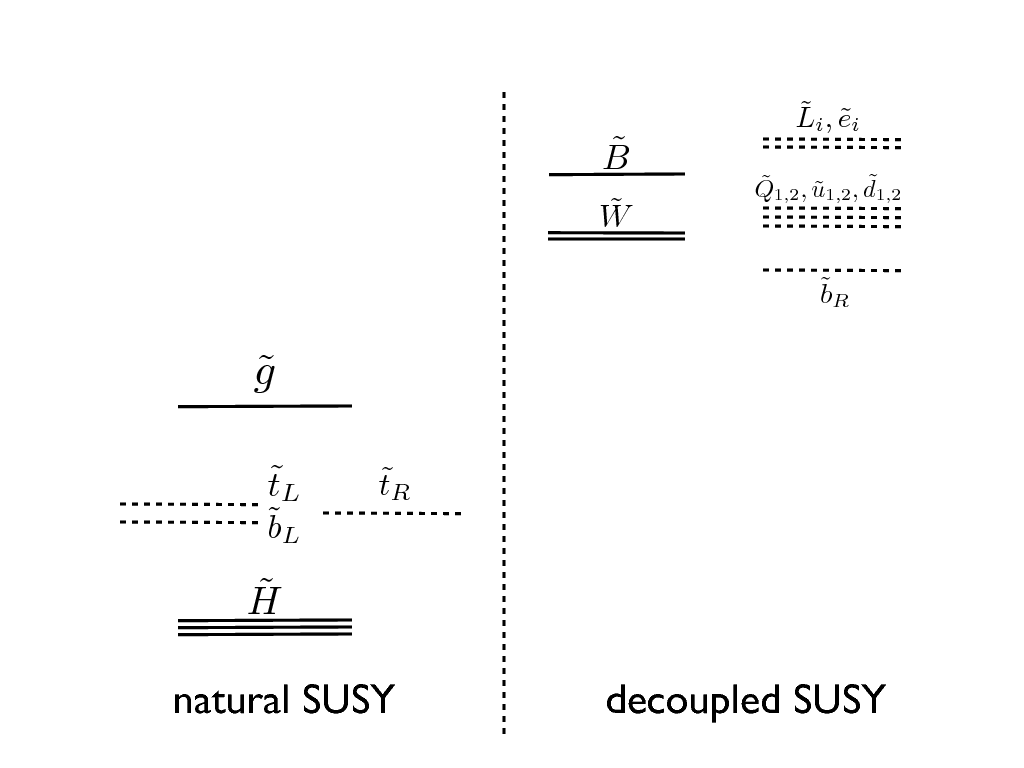
\includegraphics[angle=0,width=0.60\columnwidth]{fig/natural_susy_spectrum.png}
\end{center}
\caption{An example spectrum for natural SUSY~\cite{Papucci:2011wy}.}
\label{fig:natural_susy_spectrum}
\end{figure}

In order to gain a rough quantitative sense of what the mass constraints for these particles are, a measure of the Higgs mass fine-tuning can be constructed as
\begin{align}
\mathcal{N} \equiv \frac{\delta\mh^2}{\mh^2}.
\end{align}
Thus for $\mathcal{N} = 10$, a fine tuning of 1 part in 10, the bounds are $m_{\tilde{t}} \lesssim 1~\TeV$ and correspondingly $m_{\tilde{b}} \lesssim 1~\TeV$ and $\mglu \lesssim 2~\TeV$.

Recent results from the LHC, however, are already starting to threaten these bounds, as shown in Figure~\ref{fig:cms_susy_results} and Figure~\ref{fig:atlas_susy_results}, with gluino and stop exclusion limits already surpassing these bounds for certain models.
These constraints, however, are largely in the context of \RPC models, where a new quantum number, $P_R$, is conserved.
\RP is defined per particle as
\begin{align}
P_R \equiv (-1)^{3(B-L)+2s},
\end{align}
where $B$, $L$, and $s$ is the baryon number, lepton number, and spin of the particle.
This results in $P_R = +1$ for SM particles and $P_R = -1$ for SUSY particles.
The motivation for requiring that \RP be conserved is that the lightest supersymmetric particle (LSP), in this case, cannot decay to SM particles and is therefore stable.
For models where the LSP is a neutralino, the LSP is then a dark matter candidate.

\begin{figure}[tbp!]
\begin{center}
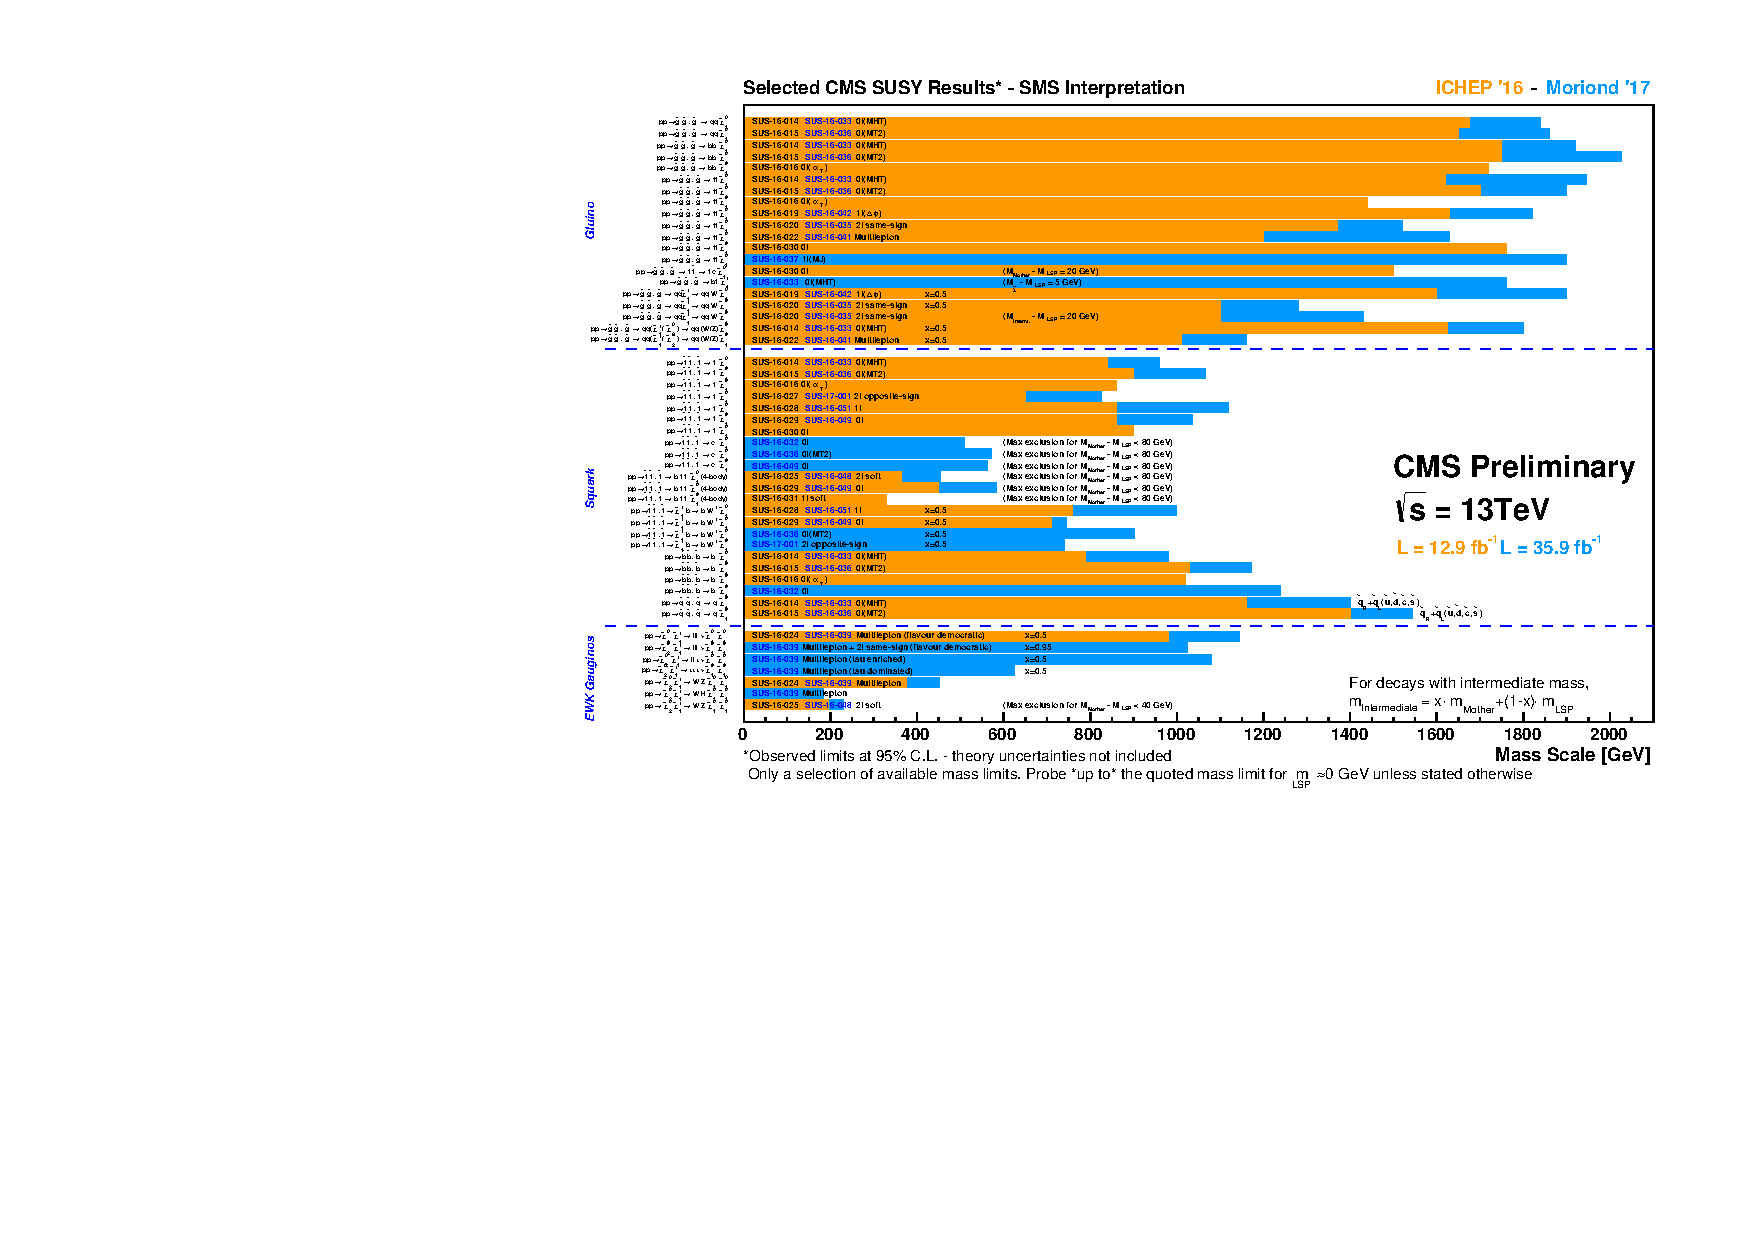
\includegraphics[angle=0,width=0.95\columnwidth]{fig/cms_susy_results.pdf}
\end{center}
\caption{An overview of recent results from SUSY searches from the Compact Muon Solenoid experiment~\cite{cms_susy_results}.}
\label{fig:cms_susy_results}
\end{figure}

\begin{figure}[tbp!]
\begin{center}
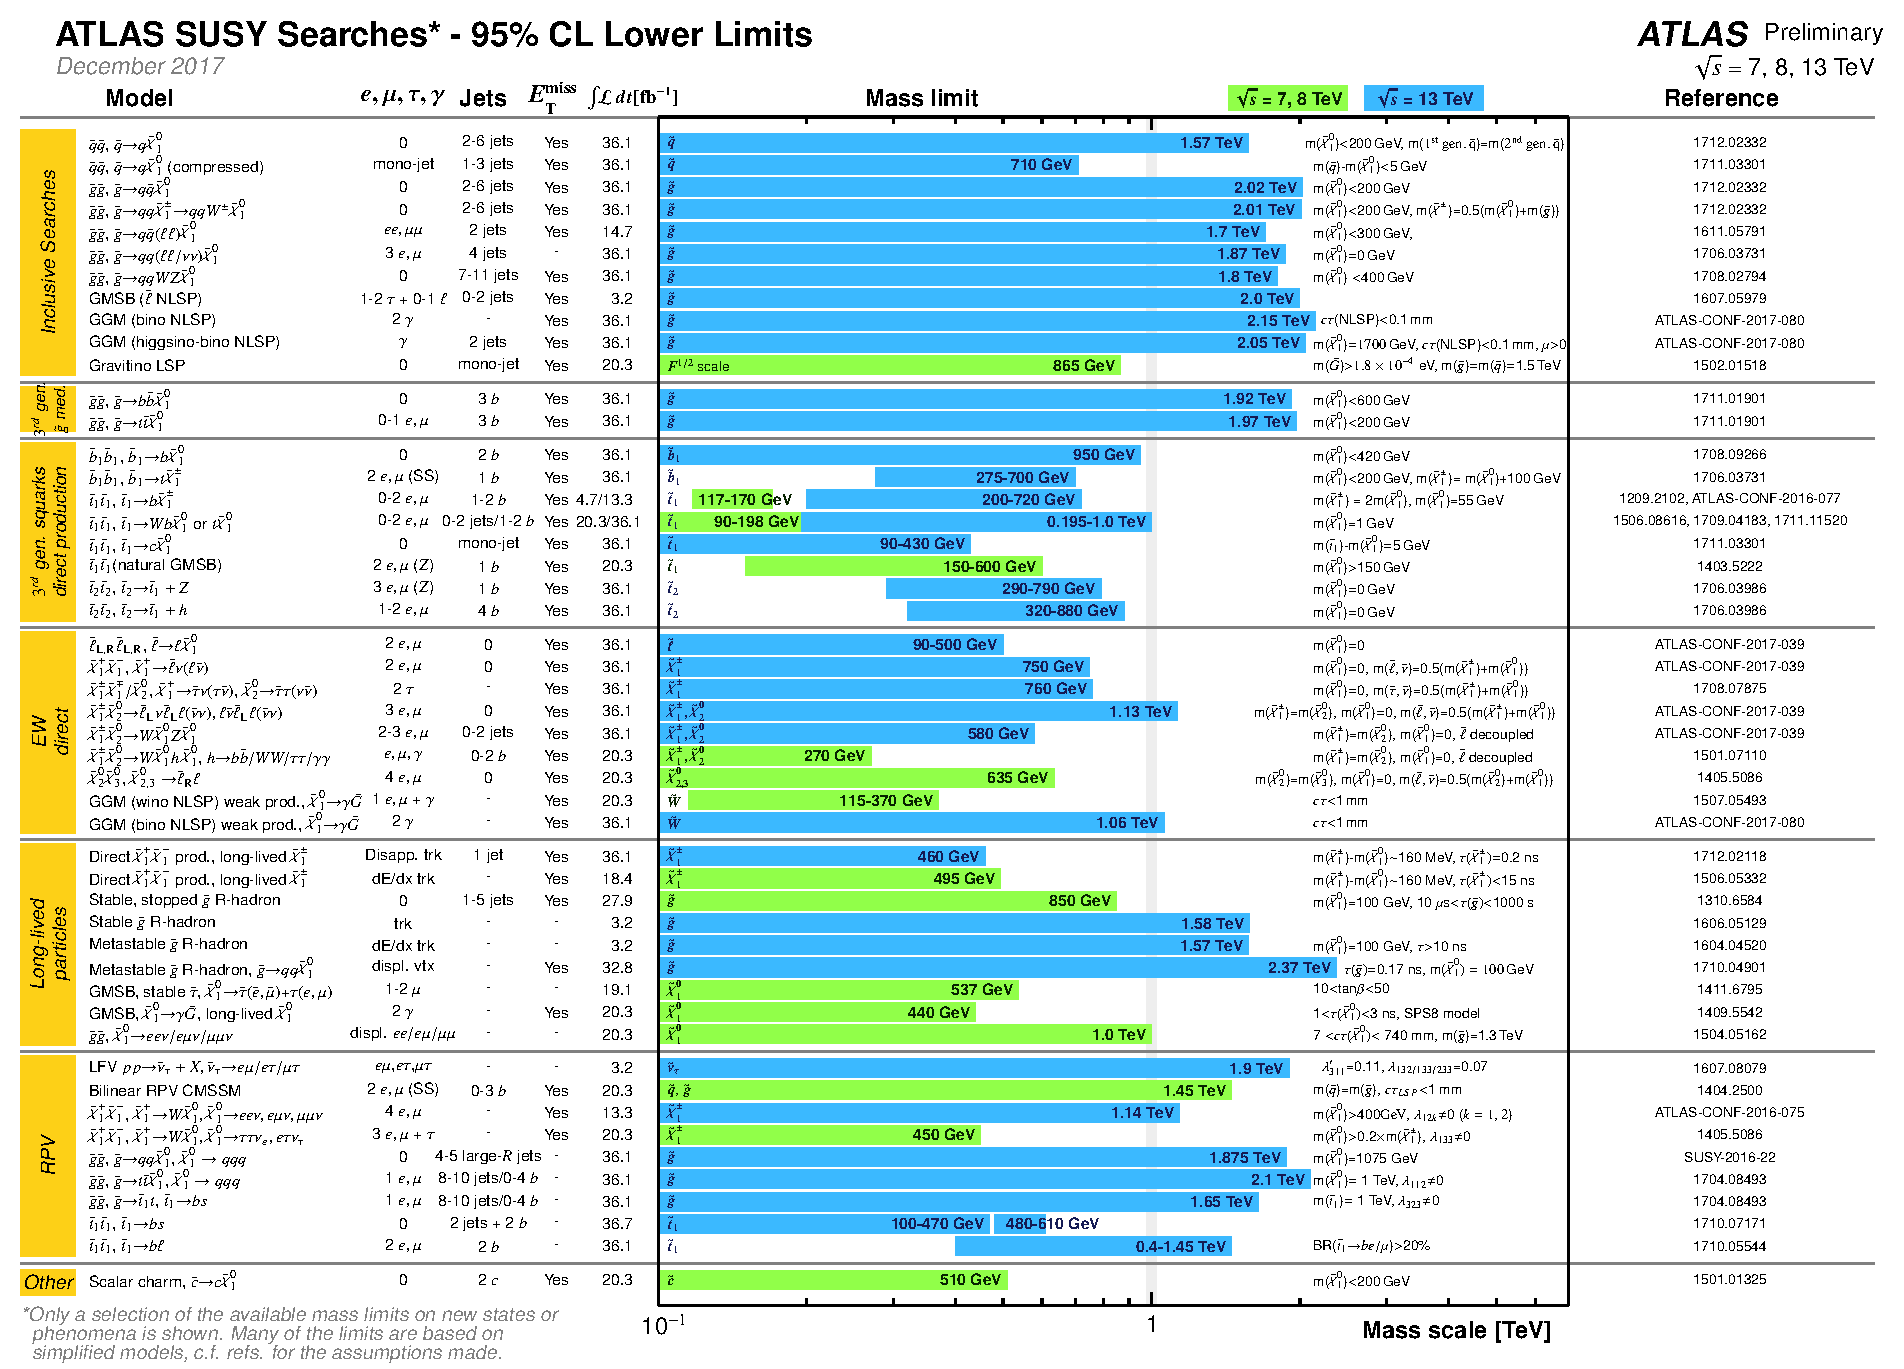
\includegraphics[angle=0,width=0.90\columnwidth]{fig/atlas_susy_results.pdf}
\end{center}
\caption{An overview of recent results from SUSY searches from the A Toroidal LHC Apparatus experiment~\cite{atlas_susy_results}.}
\label{fig:atlas_susy_results}
\end{figure}

The phenomenology, however, for \RPC (RPC) and \RPV (RPV) SUSY models is very different.
For RPC scenarios, the stable LSP does not interact with the detector and escapes without depositing any energy.
The presence of the LSPs, however, can be inferred by examining the missing transverse momentum (\MET) in an event, which due to the negligible transverse momentum of the initial colliding particles, should be 0 in events without LSPs or neutrinos.
Thus, the \MET in an event provides a powerful handle for discriminating signal and background and most analyses search for signatures that include significant amounts of \MET.
In RPV models, however, the LSP is not stable and decays to SM particles, which does not produce a large \MET signature.
Although this disfavor the LSP as a dark matter candidate, it allows RPV models to evade the constraints from RPC searches.
Subsequently, RPV SUSY yields an important class of models that can ease the tension between natural solutions to the hierarchy problem and current experimental limits.

\end{section}

\begin{section}{\RP Violating Supersymmetry}

In the MSSM, the additional \RPV terms are
\begin{align}
W_{RPV} = \frac{1}{2}\lambda^{ijk}L_{i}L_{j}\overline{\mrm{e}}_{k} + \lambda^{'ijk}L_{i}Q_{j}\overline{\mrm{d}}_{k} + \frac{1}{2}\lambda^{''ijk}\overline{\mrm{u}}_{i}\overline{\mrm{d}}_{j}\overline{\mrm{d}}_{k} + \mu^{'i}L_{i}H_{u},
\end{align}
where the color indices have been surpressed and the letters $i$, $j$, $k$ denote generation.
The fields $L_{i}$, $Q_{j}$, and $H_u$ are SU(2) doublets corresponding to leptons, quarks, and the Higgs boson, respectively, while $\overline{\mrm{e}}_k$, $u_i$, and $d_j$ are the charged lepton, up-type quark, and down-type quark SU(2) singlets.
The $\mu$ and various $\lambda$ factors are coupling strengths for their corresponding interactions, where $\lambda$ and $\lambda^{''}$ must be antisymmetric in their first and last two indices, respectively, due to color conservation.
A full description of RPV SUSY can be found in Reference~\cite{Barbier:2004ez}.

While there is no fundamental theoretical reason forbidding \RP violation, there are significant constraints on these interactions, primarilly due to the lepton number violating (LNV) couplings, $\lambda$ and $\lambda^{'}$, and and the baryon number violating (BNV) coupling, $\lambda^{''}$~\cite{Allanach:1999ic}.
The most stringent of these constraints is from proton decay on which current experimental results place a lower bound on the proton half-life of $\mathcal{O}(10^{34}\ \mrm{years})$~\cite{Bajc:2016qcc,Nishino:2009aa}.
Proton decay, however, requires both a lepton number and baryon number violating coupling, as shown in Figure~\ref{fig:proton_decay}.
This constraint can be avoided if a mechanism exists to make one of these couplings zero or negligibly small.
Additionally, though, there are strong limits on the individual LNV and BNV couplings, for example from neutron oscillation and muon-to-electron decay measurements, which are most stringent for the light generations.
Thus, for any mechanism to evade these constraints, it must also motivate smaller couplings for the lighter generations.

\begin{figure}[tbp!]
\begin{center}
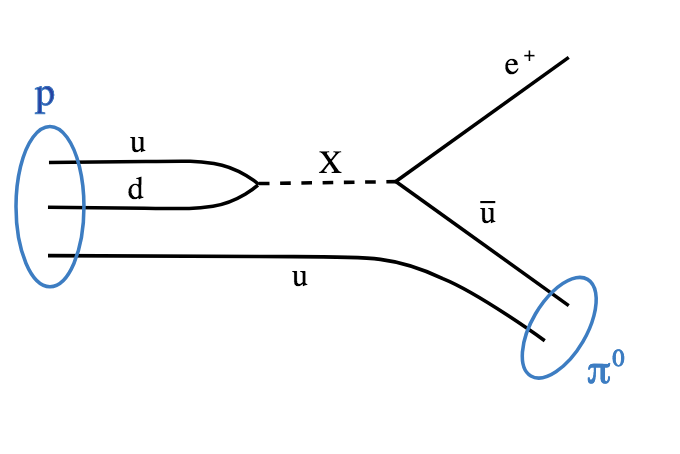
\includegraphics[angle=0,width=0.60\columnwidth]{fig/proton_decay.png}
\end{center}
\caption{Example diagram representing proton decay, where the particle X represents a down-type squark~\cite{Allanach:2016yth}.
The left vertex is mediated by the baryon number violating coupling, $\lambda^{''}$, and the right vertex is mediated by the lepton number violating coupling, $\lambda^{'}$.}
\label{fig:proton_decay}
\end{figure}

\begin{subsection}{Miminal Flavor Violating Supersymmetry}

One way to avoid the constraints placed on the RPV couplings is to construct a model by following the structure of minimal flavor violation.
In these Minimal Flavor Volating (MFV) SUSY models~\cite{Csaki:2013we,Krnjaic:2012aj,Csaki:2011ge}, the RPV couplings are related to the SM Yukawa couplings, making the third generation RPV couplings large and those of the first two small.
For example, the $\lambda^{''}$ coupling can be written as
\begin{align}
\lambda^{''}_{ijk} = w^{''} y^{(u)}_i y^{(d)}_j y^{(d)}_k \epsilon_{jkl} V^{*}_{il}
\end{align}
with $w^{''}$ an $\mathcal{O}(1)$ parameter, $y^{(u)}$ and $y^{(d)}$ the up- and down-type Yukawa couplings, and $V$ the CKM matrix.
From this, the sizes of the $\lambda^{''}_{ijk}$ couplings can be roughly estimated (using $w^{''} = 1$) and are shown in Table~\ref{tab:mfv_couplings}, which depicts the dependence of the coupling strength on generation.
Additionally, in MFV scenarios, the LNV couplings are severly suppressed by neutrino masses, and in the limit of massless neutrinos, are exactly zero.
Thus, the only relevant RPV coupling in MFV SUSY models is the BNV $\mkern1mu\overline{\mkern-1mu\mrm{u}\mkern-1mu}\mkern1mu\mkern1mu\overline{\mkern-1mu\mrm{d}\mkern-1mu}\mkern1mu\mkern1mu\overline{\mkern-1mu\mrm{d}\mkern-1mu}\mkern1mu$ coupling, which is small for the first two generations -- meeting the exact criteria necessary to evade experimental constraints on RPV couplings.
Furthermore, in the case where the LSP is a squark, it will decay promptly and not produce \MET, allowing these models to even evade the constraints from RPC SUSY searches.

\begin{table}[tbp!]
\centering
\begin{tabular}{ |c|ccc| }
\hline
     &  $ds$                 &  $db$                &  $bs$               \\
\hline
$u$  &  $3 \times 10^{-12}$  &  $6 \times 10^{-9}$  &  $5 \times 10^{-7}$ \\
$c$  &  $1 \times 10^{-8}$   &  $1 \times 10^{-5}$  &  $4 \times 10^{-5}$ \\
$t$  &  $4 \times 10^{-5}$   &  $6 \times 10^{-5}$  &  $2 \times 10^{-4}$ \\
\hline
\end{tabular}
\caption{Rough estimates for the sizes of the $\lambda^{''}_{ijk}$ MFV RPV couplings~\cite{Csaki:2011ge}.}
\label{tab:mfv_couplings}
\end{table}

Because of these considerations, MFV SUSY is an intriguing class of models to investigate experimentally.
In particular, due to the high $\glu\glu$ cross-section and large value of $\lambda^{''}_{\mrm{t}\mrm{b}\mrm{s}}$, a search for the pair-production of gluinos that decay via \rpvDecay, as shown in Figure~\ref{fig:rpv_decay}, is well-motivated.

The remainder of this dissertation is dedicated to describing such a search conducted with the Compact Muon Solenoid detector using $\sqrt{s} = 13~\TeV$ proton-proton collisions.

\begin{figure}[tbp!]
\begin{center}
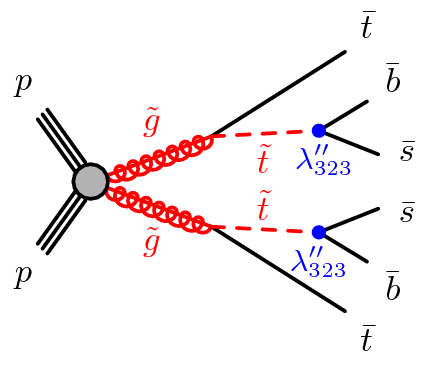
\includegraphics[angle=0,width=0.40\columnwidth]{fig/rpv_decay.png}
\end{center}
\caption{Example diagram of the pair production of gluinos that decay via \rpvDecay.}
\label{fig:rpv_decay}
\end{figure}

\end{subsection}

\end{section}
